\documentclass[11pt, a4paper]{article}
\usepackage{amsmath,amsthm, graphicx}
\usepackage{verbatim}
\usepackage{titlesec}

\titleclass{\subsubsubsection}{straight}[\subsection]

\newcounter{subsubsubsection}[subsubsection]
\renewcommand\thesubsubsubsection{\thesubsubsection.\arabic{subsubsubsection}}
\renewcommand\theparagraph{\thesubsubsubsection.\arabic{paragraph}} % optional; useful if paragraphs are to be numbered

\titleformat{\subsubsubsection}
{\normalfont\normalsize\bfseries}{\thesubsubsubsection}{1em}{}
\titlespacing*{\subsubsubsection}
{0pt}{3.25ex plus 1ex minus .2ex}{1.5ex plus .2ex}

\def\toclevel@subsubsubsection{4}
\def\l@subsubsubsection{\@dottedtocline{4}{7em}{4em}}

\title{ELEN4009 - Software Engineering\\Smart Home Power Management System\\Software Requirement Specification}
\author{Ari Croock (718005)\\Kanaka Babshet (678851)\\Alice Yang (597609)\\Daniel Weinberg (547937)}
\date{\today}
\setcounter{secnumdepth}{4}
\setcounter{tocdepth}{4}

\begin{document}
	\maketitle
	\section{Introduction}
	\subsection{Purpose}
	This document details the system requirements specification (SRS) for the Smart Home Power Management System. The system design documentation will be developed from this information.\\
	\newline 
	\noindent
	With the rapidly growing interest in new Internet of Things (IoT) technologies, networks consisting of these devices will become increasingly difficult to manage and control. Additionally, power consumption and monitoring will become a greater concern, especially in emerging markets such as South Africa.\\
	\newline 
	\noindent
	This project aims to provide a flexible software system which is able to remotely control and monitor IoT devices, as well as perform detailed power consumption diagnostics.
	
	\subsection{Project Scope}
	The project is a system that will allow for remote control, monitoring and automation of IoT devices on a Local Area Network (LAN). A client-server architecture will be used since this allows a back-end server to continuously manage devices while allowing for a client to connect on-demand. The front-end will initially be implemented as a web page for simplicity and compatibility with many existing devices (such as cellphones and personal computers). \\
	\newline 
	\noindent
	The back-end provides functionality to control and monitor devices, and to log device power consumption. Additionally, the back-end will contain the web server used for interfacing with users. \\
	\newline
	\noindent
	The front-end will consist of a web-based user interface which will provide secure access to a device dashboard. The dashboard will provide remote control and configuration of devices, as well as access to power consumption data. Addition and removal of IoT devices will also be performed through the dashboard. 
	
	\section{Project Overview}
	
	Figure~\ref{fig:dfd} shows a data flow diagram of the system. Data collected from IoT devices is stored in a database and used to control other devices as defined by the user. A web interface allows the user to configure devices and to view the stored data.
	\begin{figure}[!htb]
		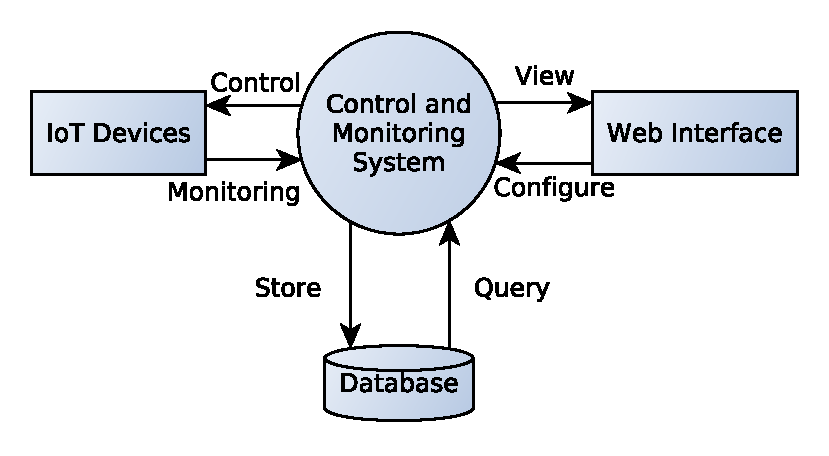
\includegraphics[width=\columnwidth]{data-flow-1}
		\caption{Data flow diagram (DFD) of the system. All data flows are bidirectional}
		\label{fig:dfd}
	\end{figure}
	\newpage
	\subsection{Assumptions}
	\begin{itemize}
		\item All of the IoT devices will be connected to the same LAN
		\item Only a small number of simultaneous users and devices will be connected at once
	\end{itemize}
	\subsection{Constraints}
	\begin{itemize}
		\item The user interface must be accessible through a web browser
		\item All devices in the system require wireless connectivity
	\end{itemize}
	
	\subsection{User Classes and Characteristics}
	\begin{itemize}
		\item Basic users who can configure basic devices and view power usage statistics
		\item Advanced users who can configure custom devices and export power usage statistics for further processing
	\end{itemize}
	
	\subsection{Operating Environment}
	The following technologies will be used to implement the system:
	\begin{itemize}
		\item Django Web Framework (Python 3.5.1)
		\item PostgreSQL Database Management System (DBMS)
		\item Docker 1.8.2
	\end{itemize}
	Assuming that few users and devices will be connected to the system simultaneously (such as in a typical household), the system requirements are fairly relaxed:
	\begin{itemize}
		\item any modern Microsoft Windows or GNU/Linux system that supports the technologies used
		\item a connection to the LAN, such as Ethernet or WiFi
		\item low-cost hardware such as a Raspberry Pi
	\end{itemize}
	However, depending on the system configuration, an external storage solution may be needed for storing a large amount of power usage data.
	
	%3 tier has better security because 2 tier the client is allowed access and communication with 
	
	\subsection{Software Development Life-cycle}
	The system will be developed using an Agile software development methodology. In particular, the popular SCRUM framework will be used so that the system's requirements and design details can change quickly if need be. 
	
	
	\section{System Features}
	The smart home power management system is made up of various features which enhance the usability of the product, along with some additional features which simplify all related functionality.
	\subsection{System Feature 1 - Remote On/Off Switching} 
	Switch any of your selected appliances on or off from any personal device connected to the home network. 
	\subsubsection{Description}
	The user can control the power status of various appliances in the household. The appliances are connected independently, for which reason, multiple appliances can be controlled through the same interface, simultaneously. 
	\subsubsection{Stimulus/Response Sequences}
	The user has to select the "Power Remote" tab on the home page to display the on and off options corresponding to each connection. 
	%\subsubsection{Functional Requirements}
	
	\subsection{System Feature 2 - User Configurable Triggers} 
	Personalise various situations which will trigger an action.
	\subsubsection{Trigger 1 - Motion Detection}
	Set appliances to switch on or off depending on surrounding motion. 
	\subsubsubsection{Description}
	The user can control whether specific appliances must be configured with motion detection or not. For example, if motion detection is set for a certain set of lights, they will detect movement in the surrounding area and switch on, or switch off when there is no motion detected for a set period of time. If the user does not want an appliance or set of lights to be triggered by motion, the respective switch is "off" on the webpage. 
	\subsubsubsection{Stimulus/Response Sequences}	
	The user has to select the "Triggers" tab from the home page, and thereafter select the "Motion Detection" tab at the top left of the newly loaded page to display the corresponding settings. Figure \ref{Trigger_Tab} in Section 4 below illustrates this page. 
	\subsubsection{Trigger 2 - Temperature Detection}
	Set appliance statuses to vary depending on the surrounding temperature.
	\subsubsubsection{Description}
	The user can control whether specific appliances must be configured with heat triggers or not. For example, if temperature detection is set for a specific appliance, it will detect a certain temperature in the surrounding area and switch on, switch off, or maintain state if it is too hot, too cold, or within the correct temperature range depending on the user choices. If the user does not want an appliance or set of lights to be triggered by the ambient temperature, the respective switch is "off" on the webpage. 
	\subsubsubsection{Stimulus/Response Sequences}	
	The user has to select the "Triggers" tab from the home page and thereafter select the "Temperature Detection" tab at the top of the newly loaded page, (second from the left), to display the corresponding settings.
	\subsubsection{Trigger 3 - Light Detection}
	Set appliance statuses to vary depending on the surrounding light.
	\subsubsubsection{Description}
	The user can control whether specific appliances must be configured with light triggers or not. For example, if light detection is set for a specific appliance, it will detect a certain ambient light level in the surrounding area and correspondingly vary, or maintain state depending on the user choices. If the user does not want an appliance or set of lights to be triggered by the ambient light levels, the respective switch is "off" on the webpage. 
	\subsubsubsection{Stimulus/Response Sequences}
	The user has to select the "Triggers" tab from the home page and thereafter select the "Light Detection" tab at the top of the newly loaded page, (third from the left), to display the corresponding settings.
	\subsubsection{Trigger 4 - Time Scheduling}
	Select and adjust times for the different appliances to be on, off, or running on defined settings. 
	\subsubsubsection{Description}
	The user can activate time scheduling for each device/set of lights independently connected to the smart home power management system. For example, the user can set the geysers to switch on from 6 am to 8 am and from 7 pm to 9 pm everyday. Note that the selection of time scheduling for appliances does not affect the user's ability to manually control the power via the system, or directly in person. 
	\subsubsubsection{Stimulus/Response Sequences}
	The user has to select the "Triggers" tab from the home page and thereafter select the "Time Scheduling" tab at the top right of the newly loaded page to display the corresponding settings.
	\subsection{System Feature 3 - Power Consumption Monitoring}
	Monitor the power consumption by various appliances and sets of lights in the household. 
	\subsubsection{Description}
	Given that this system is based on power management, the user can easily view detailed layouts of the total household power consumption data and analytics. The user will be able to view graphical statistics of the power consumption over the course of the day, as well as detailed statistics over a longer period of time (previous month, or year). This allows the user to compare the household power consumption with that of the usage if this system was not implemented. 
	\subsubsection{Stimulus/Response Sequences}
	The webpage automatically starts on the "Home Status" tab upon loading. The user can view this page for a daily consumption summary, and can then click on the "Consumption Monitoring" tab seen on the left of the same page to view these analytics in greater detail, over a longer period of time.
	\subsection{System Feature 4 - Energy Source Management}
	Control and manage the different energy sources in the household such as varying the usage between electricity and solar power. 
	\newpage
	\subsubsection{Description}
	This system encourages the use of alternative, renewable energy sources. If the user has catered for these facilities, the system allows additional power volume management through the energy source management configuration. 
	\subsubsection{Stimulus/Response Sequences}
	The user has to select the "Energy Source Management" tab on the left of the homepage to be directed to this page. 
	\subsection{System Feature 6 - User Configurable Alerts} 
	Choose which events should result in an immediate alert/notification on your system. 
	\subsubsection{Description}
	Along with all the personalised settings configured on the system, the user is able to define situations in which alerts appear on the system and possibly directly to the user's smart device. 
	\subsubsection{Stimulus/Response Sequences}
	The user has to select the "Alerts" tab on the left of the homepage to then configure these settings.
	\subsection{System Feature 7 - User Configurable Webpage Settings} 
	Define webpage settings in order to enhance the power management system experience.
	\subsubsection{Description}
	The user can add or remove devices to be controlled by the smart home power management system, alter the webpage appearance, manage users on the network, and edit security settings. 
	\subsubsection{Stimulus/Response Sequences}
	The user must click on the "Settings" link to the right of the title on the home page to be able to configure all the required settings.
	
	\section{External Interface Requirements}
	The external interface is the interface which allows the user to interact with the system through a hardware device using software. The external interfaces consists of a user interface, hardware interface, software interface and communication interface. 
	
	\subsection{User Interface - GUI}
	The user interface is how the user will interact with the system. The requirements for the design of user interface must be simple and easy to navigate. A simple format of representing all the devices connected to the Smart Home Power Management System is to display the features available for all devices on a dashboard. This can been seen in Figure \ref{Home_Dashboard}.
	
	\noindent
	Figure \ref{Trigger_Tab} is a simple illustration of the interface between the user the light detection triggers on the system. The layout of the tab is further divided to clearly illustrate the sub-systems which the user has access to. As seen from the figure, the switches on the triggers tab are designed in a graphical format that is simple for users to use.  
	
	\noindent
	Figure \ref{Settings} is the settings page, in which it designed for the user to navigate through each sub-system. The \textit{Add/Remove Device} feature is an important feature, as it is expected that the client may have to add or remove devices for future use. The settings page is set up similarly to the home page on the trigger tab, as user's  familiarity to the website is of importance.
	
	\begin{itemize}
		\item Home Page Dashboard
			\begin{figure}[!h]
				\centering
				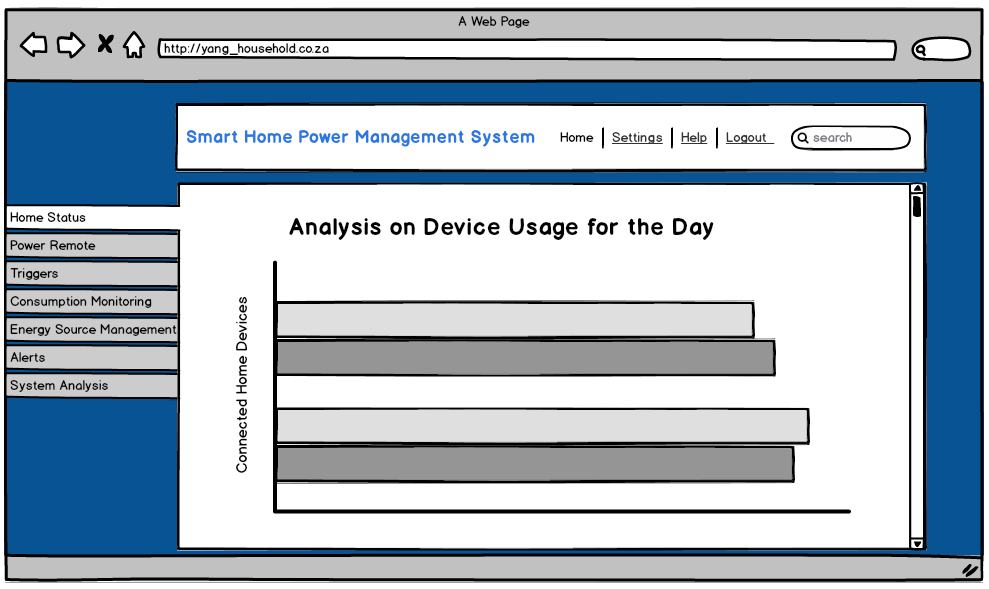
\includegraphics[scale=0.5]{Home_Page.png}
				\caption{Figure illustrating the home page the user will see once they have logged on to access the system.}
				\label{Home_Dashboard}
			\end{figure}
			\pagebreak
		\item Trigger Tab on Dashboard
			\begin{figure}[!h]
				\centering
				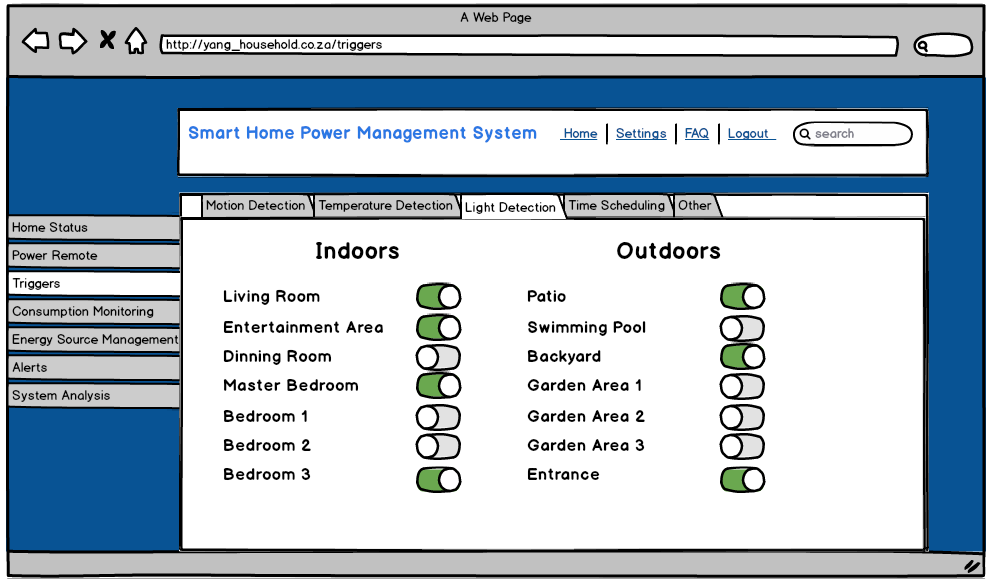
\includegraphics[scale=0.5]{Trigger_Tab.png}
				\caption{Figure illustrating the triggers tab, to allow users to control switching of sensors in their home through the system.}
				\label{Trigger_Tab}
			\end{figure}
		\item Settings Page
			\begin{figure}[!h]
				\centering
				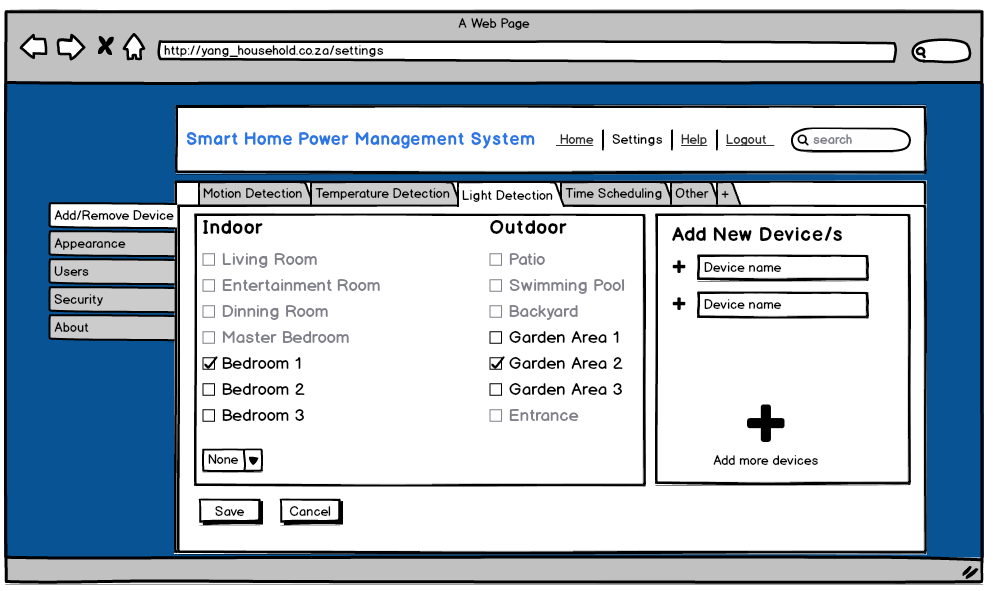
\includegraphics[scale=0.5]{Settings.png}
				\caption{Figure illustrating the settings page.}
				\label{Settings}
			\end{figure}
	\end{itemize}
	
	\pagebreak
	\subsection{Hardware Interface}
	The user interface is implemented on a web based platform that is accessible through a browser. The hardware required to access the system can be either of the listed devices found in the list below:
	
	\begin{itemize}
		\item Large Desktops (1200 -  pixels)
		\item Medium Desktops (992 - 1199 pixels)
		\item Small Devices (768 - 991 pixels)
		\item Extra Small Devices (max 767 pixels)
	\end{itemize}
	
	\subsection{Communication Interface}
	The Smart Home Power Management System is a web-based application that requires a internet connection for the communication between the hardware devices, system and IoT devices. The main connection between the system and the IoT devices is through the user's home wireless connect (WiFi). For the hardware device to communicate with the system any type of internet connection will do.
	
	\section{Other Non-Functional Requirements}
	
	\subsection{Performance Requirements}
	The smart home power system is an application and system that is designed for efficiency. This means that the application as well as the connecting household components need to respond quickly and in real time. 
	\\\\
	The application will most likely undergo several updates and changes for the user's benefit. The system is required to update on user command. Updates will include further improvements to the application as well as fixes for issues that arise in operation.
	
	\subsection{Safety Requirements} 
	The application as well as the system components need to take certain safety concerns into account. 
	\\\\
	Due to the fact that the application is essentially controlling most of a home's appliances and electricity usage, it is important that it monitors everything it is controlling to prevent problems that may arise. The application needs to ensure that any device connected in the system does not reach a dangerous level of usage. In this case, the application should either switch off the device in question or notify the user that something is not functioning correctly and needs to be addressed. 
	
	\subsection{Security Requirements}
	Due to the fact that the system controls a user's home, it therefore requires security considerations to be taken into account.
	\\\\
	The system needs to ensure that only the user has access to the application to prevent external parties gaining control of the connected components within a house. This can be done with a signup, login and authentication process. 
	The components within the house that the application connects with, need to be protected from external parties and therefore they must be explicitly authenticated. 
	
	\subsection{Software Quality Attributes}
	The application is web based and needs to be user friendly. The functioning of the application needs to be simple so that no additional documentation or prior knowledge or experience is required. 
	
	
\end{document}